% Options for packages loaded elsewhere
\PassOptionsToPackage{unicode}{hyperref}
\PassOptionsToPackage{hyphens}{url}
%
\documentclass[
]{article}
\usepackage{lmodern}
\usepackage{amssymb,amsmath}
\usepackage{ifxetex,ifluatex}
\ifnum 0\ifxetex 1\fi\ifluatex 1\fi=0 % if pdftex
  \usepackage[T1]{fontenc}
  \usepackage[utf8]{inputenc}
  \usepackage{textcomp} % provide euro and other symbols
\else % if luatex or xetex
  \usepackage{unicode-math}
  \defaultfontfeatures{Scale=MatchLowercase}
  \defaultfontfeatures[\rmfamily]{Ligatures=TeX,Scale=1}
\fi
% Use upquote if available, for straight quotes in verbatim environments
\IfFileExists{upquote.sty}{\usepackage{upquote}}{}
\IfFileExists{microtype.sty}{% use microtype if available
  \usepackage[]{microtype}
  \UseMicrotypeSet[protrusion]{basicmath} % disable protrusion for tt fonts
}{}
\makeatletter
\@ifundefined{KOMAClassName}{% if non-KOMA class
  \IfFileExists{parskip.sty}{%
    \usepackage{parskip}
  }{% else
    \setlength{\parindent}{0pt}
    \setlength{\parskip}{6pt plus 2pt minus 1pt}}
}{% if KOMA class
  \KOMAoptions{parskip=half}}
\makeatother
\usepackage{xcolor}
\IfFileExists{xurl.sty}{\usepackage{xurl}}{} % add URL line breaks if available
\IfFileExists{bookmark.sty}{\usepackage{bookmark}}{\usepackage{hyperref}}
\hypersetup{
  hidelinks,
  pdfcreator={LaTeX via pandoc}}
\urlstyle{same} % disable monospaced font for URLs
\usepackage{graphicx,grffile}
\makeatletter
\def\maxwidth{\ifdim\Gin@nat@width>\linewidth\linewidth\else\Gin@nat@width\fi}
\def\maxheight{\ifdim\Gin@nat@height>\textheight\textheight\else\Gin@nat@height\fi}
\makeatother
% Scale images if necessary, so that they will not overflow the page
% margins by default, and it is still possible to overwrite the defaults
% using explicit options in \includegraphics[width, height, ...]{}
\setkeys{Gin}{width=\maxwidth,height=\maxheight,keepaspectratio}
% Set default figure placement to htbp
\makeatletter
\def\fps@figure{htbp}
\makeatother
\setlength{\emergencystretch}{3em} % prevent overfull lines
\providecommand{\tightlist}{%
  \setlength{\itemsep}{0pt}\setlength{\parskip}{0pt}}
\setcounter{secnumdepth}{-\maxdimen} % remove section numbering

\date{}

\begin{document}

\hypertarget{cloud-to-sensors-field-level-connectivity}{%
\section{Cloud to Sensors Field Level
Connectivity}\label{cloud-to-sensors-field-level-connectivity}}

\hypertarget{architecture}{%
\subsection{Architecture}\label{architecture}}

\hypertarget{introduction}{%
\subsubsection{Introduction}\label{introduction}}

As it was explained in Sect 1, to follow the Industry 4.0 concept a
hybrid environment integrating reactive Machine to Machine
interconnection and interactive web-based user interface is required.
The main challenge of the solution in concern is to design a generic but
reusable architecture that addresses interoperability of these diverse
interconnection scenarios ruled by different requirements, namely

\begin{enumerate}
\def\labelenumi{\arabic{enumi}.}
\tightlist
\item
  \textbf{machine-centric} machine to machine real-time mobile
  interoperability
\item
  \textbf{human-centric} cloud-based front-end
\end{enumerate}

Interconnection of the reactive \textbf{machine-centric} and interactive
\textbf{human-centric} environments can be implemented by applying one
of the following scenarios:

\begin{itemize}
\tightlist
\item
  \textbf{direct interconnection} - cloud-based dedicated communication
  services are engaged to attach it to the cyber-physical system making
  up a consistent M2M communication network using a common protocol
  stack
\item
  \textbf{gateway based interconnection} - native build-in communication
  services allows attaching the cloud to the cyber-physical system using
  an out-of-bound protocol stack
\end{itemize}

In the solution in concern, the interconnection of assets is not enough
hence their interoperability is expected. In this case, using the same
communication stack must be recognized as only a necessary condition. To
support interoperability common data understanding is required. By
design, the direct approach requires that the cloud has to be compliant
with the interoperability standard the cyber-physical system uses. As a
result, it becomes a consistent part of the cyber-physical system.
Additionally, to meet this requirement the cloud and cyber-physical
systems have to establish

\begin{itemize}
\tightlist
\item
  directly the same semantic-context
\item
  directly the same security-context
\end{itemize}

The possibility to establish a common semantic-context in the
multi-vendor environment makes communication standardization especially
important. In this case, it is required that the encoding of the payload
of messages exchanged over the network (Data Transfer Object - TDO) is
standardized so that the payload can be factored on the data-gathering
site and consumed on the ultimate destination data processing sites.
Security between the data origin and ultimate data destination refers to
the protection of messages (security-context) against malicious users.
It is required that communicating parties are using the same
cyber-security measures.

\hypertarget{why-not-direct}{%
\subsubsection{why not direct}\label{why-not-direct}}

The decision to follow the \textbf{direct interconnection} scenario must
be derived from an analysis of the capabilities of available services in
concern. However, for the development strategy of this type of solutions
this analysis can be done partially taking into account two features
that can be considered invariable:

\begin{itemize}
\tightlist
\item
  by design the cloud-based services must be virtual - they are used to
  handle many solutions at the same time
\item
  by design the M2M communication is usually constrained by the
  real-time requirements
\end{itemize}

In practice, the set of assets embedded in the cyber-physical system is
very stable. On the another hand, the virtualization of services means
that they must be very flexible to handle the attachment of new assets
proactively (acting in advance) at run time. As a result, by design, the
cloud services must be repressible to register and authenticate devices
exposing endpoints in the public network to allows the device to access
a provisioning cloud service. It requires that a session over the
Internet has to be established by the data holding asset at a
preparation step.

To meet the requirements of real-time distributed control the
cyber-physical system may use protocols applicable only to local
computer networks (e.g.~multicast IP, Ethernet, TSN, etc.). Because the
cloud services support only protocols handling interconnection over the
Internet the interaction with the cloud requires remote agents,
i.e.~agents attached locally to the M2M network implemented applying one
of the following archetypes:

\begin{itemize}
\tightlist
\item
  \textbf{edge device} - remote cloud agent acting as an intermediary
  for nodes of the cyber-physical network
\item
  \textbf{field level gateway} - a dedicated custom device acting as an
  intermediary for nodes of the cyber-physical network
\item
  \textbf{embedded gateway} - a software part composed into a selected
  node of the cyber-physical network
\end{itemize}

\textbf{Edge device} is a device that connects directly to the cloud
services but acts as an intermediary for other devices called leaf
devices. Additionally, it allows the selection of initial data
processing and execution of them using local resources. The \textbf{edge
device} may be located close to the leaf devices and attached to the
cyber-physical network using protocols applicable only to local computer
networks. In this scenario, it is possible to use a custom protocol
stack to get connected to the \textbf{edge device} with the cloud and
helps to save the bandwidth thanks to sending only the results of local
processing. In this approach, the \textbf{edge device} is part of cloud
vendor products and cannot be recognized as a generic solution that can
be used to connect to other clouds at the same time.

The \textbf{field level gateway} is also build atop of the middleware
concept. The only difference compared with the \textbf{edge device} is
necessity to use officially supported by the cloud vendor services to
get connected. In this scenario the process data may be transferred to
many clouds at the same time provided that the gateway offers this
functionality.

\begin{figure}
\centering
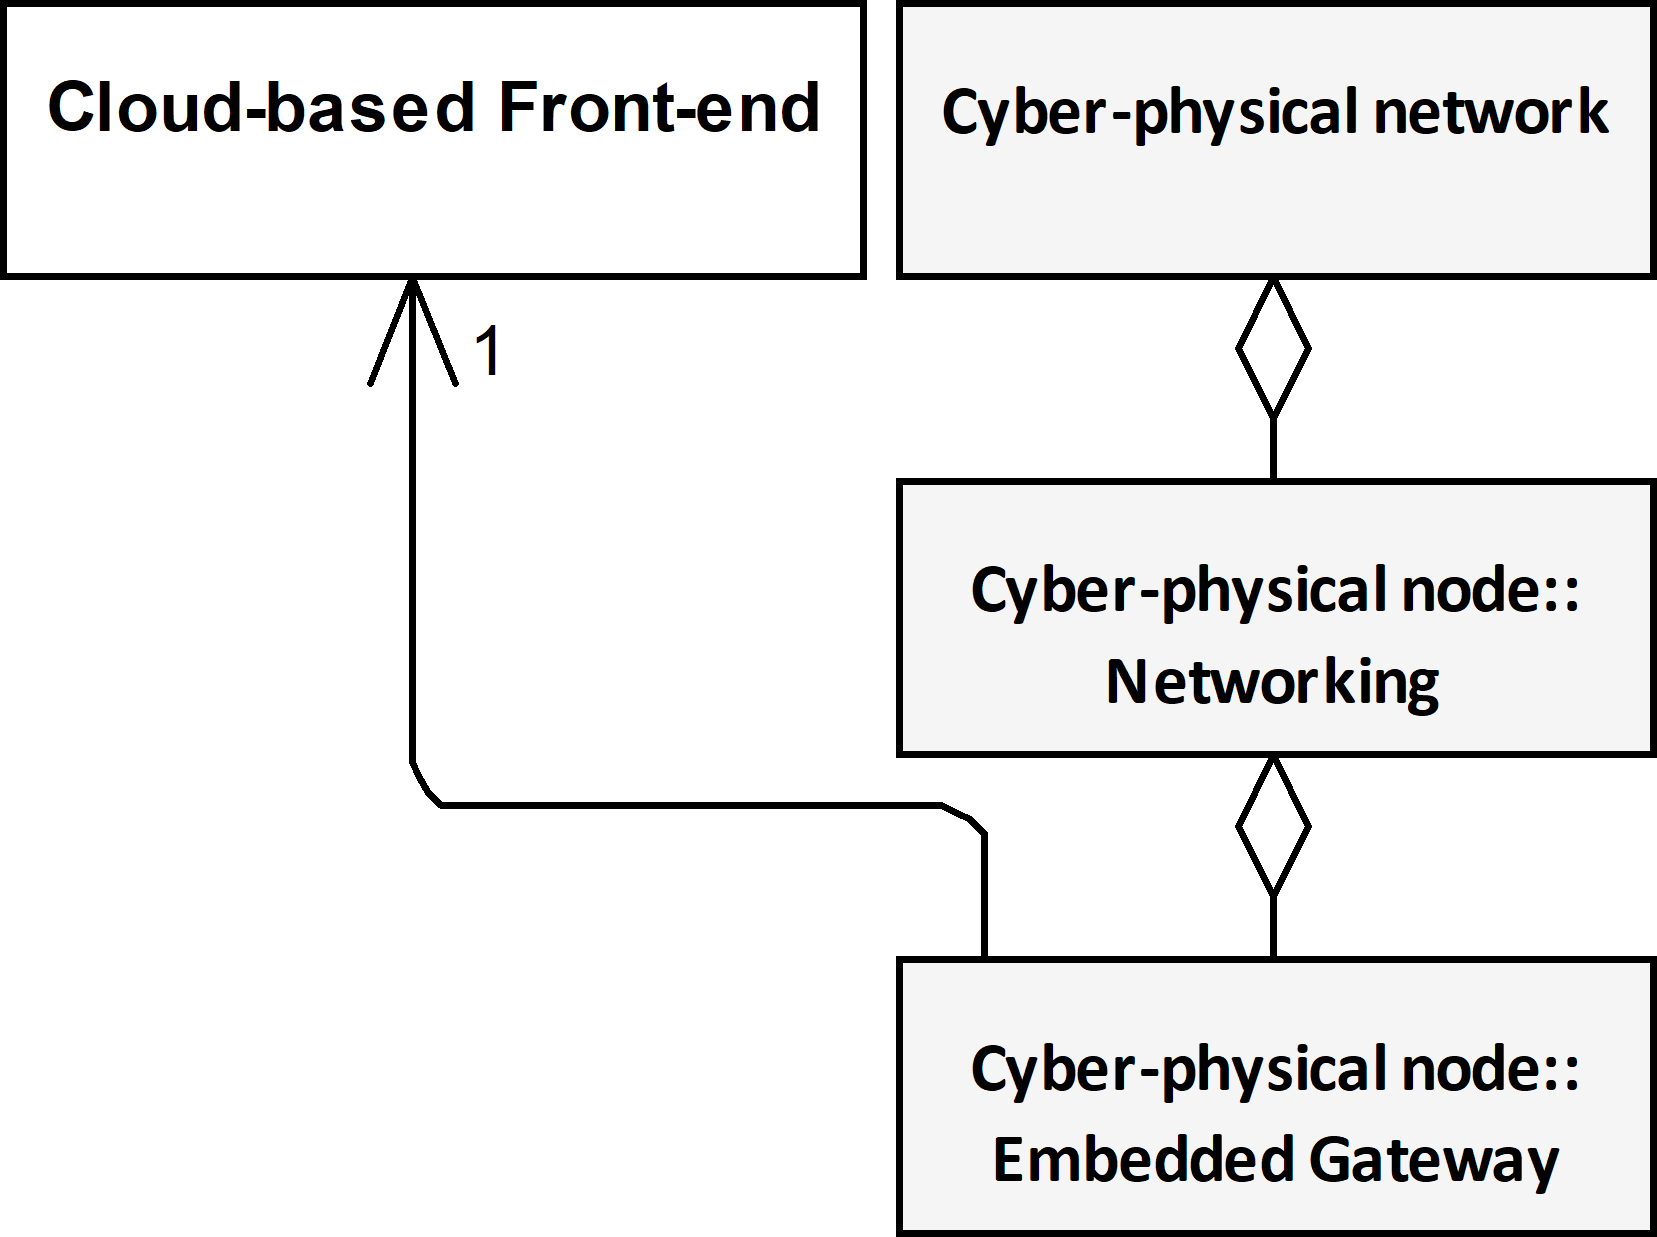
\includegraphics{../.Media/StrategyDomainModel.png}
\caption{Strategy Domain Model}
\end{figure}

Unlike the above described solutions, the \textbf{embedded gateway} is
not derived from the middleware concept. The domain model for this
archetype is presented in the Fig. Promoting separation of concern
design principle, the gateway functionality should be implemented as a
self-contained software part embedded in the \texttt{Networking} service
of the \texttt{Cipher-physical\ node}. Main functionality of this
component is to transfer selected data between
\texttt{Cipher-physical\ network} using \texttt{Networking} services of
an existing \texttt{Cipher-physical\ node} and
\texttt{Cloud-based\ front-end} using officially supported by the cloud
vendor interconnection services.

The \textbf{embedded gateway} archetype relaxes most of the issues
described above: cipher-physical network real-time behavior, data
encoding incompatibility, security-context differences to name only a
few. The main goal of this article is to provide proof that the
\textbf{embedded gateway} archetype implementation is possible based on
a generic architecture that can be used as a foundation for the
integration of the heterogenous environments in concern. The proposed
implementation is designed for selected interoperability standard and
cloud product.

\hypertarget{why-pubsub}{%
\subsection{Why pubsub}\label{why-pubsub}}

To comply with the Industry 4.0 communication criterion, even the lowest
category requires that the product must be addressable over the network
via TCP/UDP or IP and has to support the OPC UA Information Model. As a
result, any product being advertised as Industry 4.0 enabled must be OPC
UA-capable somehow. To support the multi-vendor environment OPC Unified
Architecture interoperability standard has been selected. OPC UA
supports the following two patterns to be used to transfer data between
communicating parties:

\begin{itemize}
\tightlist
\item
  connection-oriented: requires a session that has to be established
  before any data can be sent between sender and receiver
\item
  connectionless-oriented: the sender may start sending messages (called
  packets or datagrams) to the destination without any preceding
  handshake procedure
\end{itemize}

Using the connection-oriented communication pattern it is difficult or
even impossible to gather and process mobile data (Sec. I), which is one
of the Internet of Things paradigms. OPC UA Part 14 PubSub offers the
connectionless approach as an additional option to session based
client-server interoperability and is a consistent part of the OPC UA
specifications suit. As the result it can be recognized as the IoT ready
technology.

\begin{quote}
{[}29{]} Mariusz Postol, UA Part 14: PubSub Main Technology Features in
Object Oriented Internet, https://github.com/mpostol/OPC-UA-OOI, 2019,
DOI: 10.5281/zenodo.1198852
\end{quote}

\hypertarget{why-azure}{%
\subsection{Why Azure}\label{why-azure}}

The presented proposals in the article are backed by proof of concept
reference implementations. For this study, prototyping addresses
Microsoft Azure cloud products. There are many reasons for selecting
Azure to accomplish cloud-based front-end of CFS. Azure offers
Infrastructure as a Service (IaaS) and Platform as a Service (PaaS)
capabilities. As a result, the platform can be used not only as a
cloud-based front-end for CFS. By design, the Azure services are
compliant with Security Development Lifecycle (SDL) an industry-leading
security process. It is also compliant with the new international
standard for cloud privacy, namely ISO 27018. Solutions hosted on Azure
are scaled up to millions of users without any additional coding. For
the development of the CFS front-end, it is essential that Azure
provides very efficient storage services usefully for real-time process
data archival. Azure provides a vast variety of hybrid connections
including but not limited to virtual private networks (VPNs), caches,
content delivery networks (CDNs), ExpressRoute, and IoT dedicated
services that can be directly used to implement cloud-based front-end
for CFS. Because it is also integrated with other Microsoft tools like
Office 365, Outlook, and SharePoint using Azure allows preserving
investment and exporting process data to the mentioned tools. Azure also
offers services supporting analytics and intelligence capabilities for
further improving business processes and decision making. It is the only
cloud platform that offers Blockchain as a Service (BaaS), Machine
Learning, Bots, and Cognitive APIs capabilities.

Azure aids Internet protocols and open standards such as JSON, XML,
SOAP, REST, MQTT, AMQP, and HTTP. A software development kits for C\#,
Java, PHP, and Ruby are available for custom applications. Azure
provides services supporting data exchange over the OPC UA, but they
don't support pubsub compliant with the OPC UA Part-14. Connectivity
services on the network use JSON-based Data Transfer Object encoded
based on schema derived from the solution metadata.

More detailed description of the selected Azure features in context of
the application in concern are covered by the Sec.
\texttt{azure-main-technology-features}.

\hypertarget{why-ooi}{%
\subsection{Why OOI}\label{why-ooi}}

Based on the sessionless and session-oriented communication patterns
examination against the IoT requirements (cite mpostol 2020) it could be
concluded that the connectionless pattern better suites issues related
to the assets mobility and traffic asymmetry that is characteristic for
the application domains in concern. Additionally, to promote
interoperability and address the demands of the M2M communication in the
context of a multi-vendor environment the prototyping should use an
framework that must be compliant with the OPC UA Part 14 PubSub spec.
According to proposed architecture presented in Fig. above to implement
the \texttt{Embedded\ Gateway} as a composable part of the
\texttt{Cipher-physical\ Node} a library implementing
\texttt{Networking} functionality in compliance with mentioned above
specification is a starting point for further development. Additionally
it must be assumed that the library used to deploy
\texttt{Embedded\ Gateway} support dependency injection and be capable
to compose an external part supporting Azure/pubsub gateway
functionality. The composition process must be available without
modification of the core code of an existing library. As a result the
prototyping is to be limited to implementation of the
\texttt{Embedded\ Gateway} software part only.

A library that meets all these requirements has been implemented
consistently with the Object-Oriented Internet paradigm
\texttt{\textbackslash{}footnote\{\textbackslash{}url\{https://github.com/mpostol/OPC-UA-OOI\}\}}
\texttt{\textbackslash{}cite\{RefWorks:doc:5c66740ae4b081adf5804596\}}
worked out in an open-source project. The
\texttt{cite\ \{mpostol\ 2020\}} covers the description of a reference
application program implementation proving that it is possible to design
universal architecture targeting reactive interoperability as a
consistent part of the Object-Oriented Internet concept compliant with
the OPC UA PubSub
\texttt{\textbackslash{}cite\{RefWorks:doc:5d98837de4b055984c0eecf0\}}
international standard. According to the presented implementation and
evaluation, using the dependency injection and late binding, the
application program can be seamlessly adapted to the production
environment and scales well. This approach also improves flexibility and
adaptability of the existing solutions against any modification of the
production environment including but not limited to the selected
interoperability standard change.

Sect. \texttt{OPC\ UA\ PubSub\ Main\ Technology\ Features} provides more
detailed description of this library and new functionality
(\texttt{Embedded\ Gateway} part deployment process.

The following subsections covers description of the current state of
technologies with regards to OPC UA pubsub and Azure cloud-based IoT
enabler.

\hypertarget{review-of-technologies}{%
\subsection{Review of Technologies}\label{review-of-technologies}}

add here subsections related to the Azure and OOI

\end{document}
